\documentclass{ximera}

\title{Implicit Differentiation Activity Solution Guide}
\author{MATH 425: Calculus I}

\begin{document}
\begin{abstract}
    Working with the peers in your group, solve the following problems. Make sure to show and justify all your work. Make sure everyone in the group understands the solution and participates. Be prepared to report your answers to the whole class. 
\end{abstract}
\maketitle


\begin{exercise}
    Consider the curve on the graph and the equation of the curve: 
    $$x=y^5-5y^3+4y.$$
    With your group, explain how you would answer the following questions, using both the graph of the curve and the symbolic equation.
    \begin{image}
    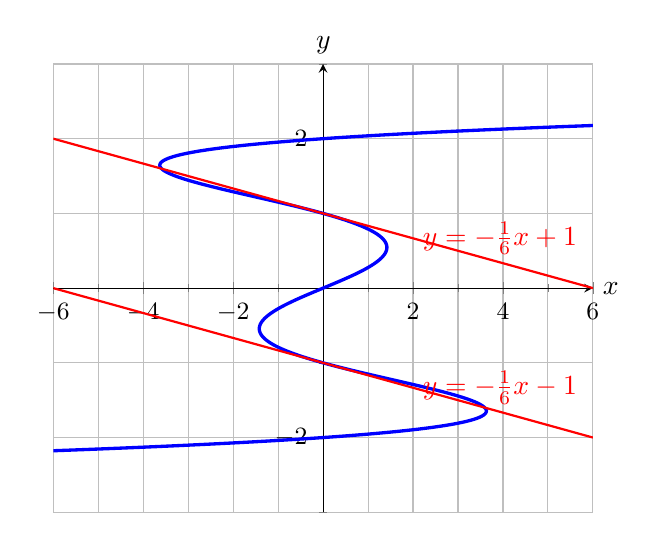
\begin{tikzpicture}
  \begin{axis}[
    axis lines=middle,
    xlabel={$x$},
    ylabel={$y$},
    xmin=-6, xmax=6,
    ymin=-3, ymax=3,
    grid=both,
    minor tick num=1,
    enlargelimits=false,
    ticklabel style={font=\small},
    every axis x label/.style={at={(current axis.right of origin)}, anchor=west},
    every axis y label/.style={at={(current axis.above origin)}, anchor=south},
  ]

    \addplot[
      domain=-2.5:2.5,
      samples=500,
      very thick,
      blue
    ] ({x^5 - 5*x^3 + 4*x}, {x});
    
    % Line y = -(1/6)x + 1
    \addplot[
      domain=-6:6,
      samples=200,
      red,
      thick,
    ] { -1/6 * x + 1 };

    % Optional: label the line
    \node[red, anchor=west] at (axis cs:2, -1/6*2 +1) {$y=-\frac{1}{6}x+1$};

     % Line y = -(1/6)x - 1
    \addplot[
      domain=-6:6,
      samples=200,
      red,
      thick,
    ] { -1/6 * x - 1 };

    % Optional: label the line
    \node[red, anchor=west] at (axis cs:2, -1/6*2 -1) {$y=-\frac{1}{6}x-1$};
  \end{axis}
\end{tikzpicture}
    \end{image}
    %\xmalt{A graph of $x=y^5-5y^3+4y$ with tangent lines $y=\frac16x-1$ at $(0,-1)$ and $y=-\frac16x+1$ at $(0,1)$.}
  \begin{enumerate}
    \item Is it possible to express $y$ as an explicit function of $x$?  
    \begin{enumerate}
        \item Explain your response using the graph.\\
        \textcolor{blue}{No, the function cannot be written as an explicit function of $x$, because it does not pass the vertical line test. (There are multiple outputs for some inputs.)}
        \item Explain using the symbolic equation for the curve $x=y^5-5y^3+4y$.\\
        \textcolor{blue}{Though we can factor out a $y$ from the right side, we cannot fully solve for $y$ in terms of $x$.  }
    \end{enumerate}
    \item Use implicit differentiation to find a formula for $\frac{dy}{dx}$.  \\
    \textcolor{blue}{
      \[\frac{d}{dx}(x)=\frac{d}{dx}(y^5-5y^3+4y)\]
      \[1=5y^4\frac{dy}{dx}-15y^2\frac{dy}{dx}+4\frac{dy}{dx}\]
      \[1=\frac{dy}{dx}(5y^4-15y^2+4)\]
      \[\frac{dy}{dx}=\frac{1}{5y^4-15y^2+4}\]
    }
    \item Explain the meaning of $\frac{dy}{dx}$.  What does it represent?\\
    \textcolor{blue}{The derivative is the instantatneous change of the curve at a point $(x,y)$. (Or the slope of the tangent line to the curve at the point $(x,y)$.)}
    \item Sam noticed that his expression for $\frac{dy}{dx}$ does not contain $x$.  Sam thinks this means that the rate of change is constant for all points on the $x$-axis.  Is Sam correct in his thinking or not? Explain.\\
    \textcolor{blue}{Since the derivative expression does include $y$, and points on the $y$-axis have form $(0,y)$, the derivative will change based on points. Also, since this is a function of $x$ with respect to $y$, there is only one $x$ value for each $y$.}
    \item Find the equation of the line tangent to the graph of $x=y^5-5y^3+4y$ at the point $(0,1)$.  Add a sketch of the tangent line to the graph.\\
    \textcolor{blue}{Slope: sub $x=0$ and $y=1$ into the derivative \\
    \[\frac{dy}{dx}=\frac{1}{5(1)^4-15(1)^2+4}=-\frac{1}{6}\]
    Tangent line: $y-1=-\frac16(x-0)$ or $y=-\frac16x+1$}
    \item Are there other points on the graph where the tangent line is the parallel to the one you found in (e)?  Respond using the graph, then verify algebraically.\\
    \textcolor{blue}{It appears from the graph that the point $(0,-1)$ would have the same slope.  To verify, sub this point into the derivative:\\
    \[\frac{dy}{dx}=\frac{1}{5(-1)^4-15(-1)^2+4}=-\frac{1}{6}\]}
    \item Determine all points at which the graph of $x=y^5-5y^3+4y$ has a vertical tangent line.  How many such points are there?  Explain your reasoning, and locate the points on the graph.\\
    \textcolor{blue}{Vertical tangent lines have undefined slope. $\frac{dy}{dx}$ is undefined when the denominator is 0.
    \[0=5y^4-15y^2+4\]
    Use the quadratic formula: 
    \[y^2=\frac{15\pm\sqrt{(-15)^2-4(5)(4)}}{2(5)}=1.5\pm\frac{\sqrt{145}}{10}\]
    \[y=\pm1.644, \pm0.544\]}
  \end{enumerate}
\end{exercise}

Problem adapted from Boelkins, Austin \& Schlicker, (2018) \textit{Active Calculus 2.1}.

\begin{exercise}
  Consider the expression $x^2+xy+y^2=3$. 
    \begin{center}
      \desmos{yey6o1coa2}{800}{600}
    \end{center}
    \begin{enumerate}
      \item Use implicit differentiation to find $y'$ (also known as $\frac{dy}{dx}$).  \\
      \textcolor{blue}{Take the derivative of both sides with respect to $x$:
      \[2x+xy'+y+2yy'=0\]
      \[2x+y=-xy'-2yy'\]
      \[2x+y=y'(-x-2y)\]
      \[y'=\frac{2x+y}{-x-2y}\]}
      \item Find the tangent line to $x^2+xy+y^2=3$ at the point $(-1,-1)$.  Sketch the tangent line on the graph (in Desmos) and check your equation is consistent with what you expect.  \\
      \textcolor{blue}{Slope: $y'\bigg|_{(-1,-1)}=\frac{2(-1)+(-1)}{-(-1)-2(-1)}=-1$\\
      Tangent line: $y+1=-(x-1)$\\
      You can type the graph into the Desmos linked above or your own Desmos graph to check.}
      \item Find any points where the tangent line to the curve is horizontal using the graph.  Sub these points into the derivative to confirm the result.\\
      \textcolor{blue}{By inspection of the graph, it appears the curve is horizontal at the points $(1,-2)$ and $(-1,2)$. \\
      Check: $y'\bigg|(-1,2)=\frac{2(-1)+2}{1-2(2)}=\frac{0}{-3}=0$\\
      $y'\bigg|(1,-2)=\frac{2(1)-2}{-1-2(-2)}=\frac{0}{3}=0$}
    \end{enumerate}
\end{exercise}

% \begin{exercise}
%     Consider the equation whose graph is given below: 
%     $$y(y^2-1)(y-2)=x(x-1)(x-2)$$
%     \begin{center}
%       \desmos{nevnd0z4lp}{800}{600}
%     \end{center}
%    %\[ \graph{y(y^2-1)(y-2)=x(x-1)(x-2)}   \]
% % Need a workaround for PDF version
%   \begin{enumerate}
%     \item Examine the graph of the curve and determine at how many points the tangent to the curve is horizontal.  Add the sketch of the horizontal tangent lines to the graph. \\
%     \textcolor{blue}{There are eight points where the tangent line is horizontal. (See graph)}
%     \item Through implicit differentiation, it can be shown that 
%       \[\frac{dy}{dx}=\frac{(x-1)(x-2)+x(x-2)+x(x-1)}{(y^2-1)(y-2)+2y^2(y-2)+y(y^2-1)}\]
%       Determine all of the $x$-values of points at which the tangent line to the curve is horizontal.  Compare the result of your calculation to the answer you got in question (a).  If they seem not to agree, can you explain why they may not appear to match? \\
%       \textcolor{blue}{$\frac{dy}{dx}=0$ when the numerator is equal to 0:\\
%       \[(x-1)(x-2)+x(x-2)+x(x-1))=x^2-3x+2+x^2-2x+x^2-x=3x^2-6x+2=0\]
%       \[x=\frac{6\pm\sqrt{(-6)^2-4(3)(2)}}{2(3)}\approx 1.57735,0.42265\]
%       }
%     \item Determine all the $y$-values of points at which the tangent line to the curve is vertical.  You may use a graphing calculator or Desmos to solve the polynomial involved. \\
%     \textcolor{blue}{We need to find where the denominator is 0, so put the denoinator into a graphing calculator or desmos ($x=(y^2-1)(y-2)+2y^2(y-2)+y(y^2-1)$.  The zeroes are $x=-0.618,0.5,1.618$.)}
%     \item Find the equation of the tangent line to the curve at one of the points where $x=1$.\\
%     \item   \textcolor{blue}{Choose one of $(1,2)$, $(1,1)$, $(1,0)$, $(1,-1)$:\\
%     For $(1,2)$:\\
%     Slope: $\frac{(1-1)(1-2)+1(1-2)+1(1-1)}{(2^2-1)(2-2)+2(2)^2(2-2)+2(2^2-1)}=-\frac{1}{6}$\\
%     Tangent line: $y-2=-\frac16(x-1)$\\
%     For $(1,1)$:\\
%     Slope: $\frac{(1-1)(1-2)+1(1-2)+1(1-1)}{(1^2-1)(1-2)+2(1)^2(1-2)+1(1^2-1)}=\frac12$\\
%     Tangent line: $y-1=\frac12(x-1)$\\
%     For $(1,0)$:\\
%     Slope: $\frac{(1-1)(1-2)+1(1-2)+1(1-1)}{(0^2-1)(0-2)+2(0)^2(0-2)+0(0^2-1)}=-\frac12$\\
%     Tangent line: $y=-\frac12(x-1)$\\
%     For $(1,-1)$:\\
%     Slope: $\frac{(1-1)(1-2)+1(1-2)+1(1-1)}{((-1)^2-1)(-1-2)+2(-1)^2(-1-2)+(-1)((-1)^2-1)}=\frac16$\\
%     Tangent line: $y+1=\frac16(x-1)$\\
%     }
%   \end{enumerate}
% \end{exercise}







\end{document}